\chapter{Diseño e implementación} % Main chapter title

\label{Chapter3} % Change X to a consecutive number; for referencing this chapter elsewhere, use \ref{ChapterX}

\definecolor{mygreen}{rgb}{0,0.6,0}
\definecolor{mygray}{rgb}{0.5,0.5,0.5}
\definecolor{mymauve}{rgb}{0.58,0,0.82}

%%%%%%%%%%%%%%%%%%%%%%%%%%%%%%%%%%%%%%%%%%%%%%%%%%%%%%%%%%%%%%%%%%%%%%%%%%%%%
% parámetros para configurar el formato del código en los entornos lstlisting
%%%%%%%%%%%%%%%%%%%%%%%%%%%%%%%%%%%%%%%%%%%%%%%%%%%%%%%%%%%%%%%%%%%%%%%%%%%%%
\lstset{ %
  backgroundcolor=\color{white},   % choose the background color; you must add \usepackage{color} or \usepackage{xcolor}
  basicstyle=\footnotesize,        % the size of the fonts that are used for the code
  breakatwhitespace=false,         % sets if automatic breaks should only happen at whitespace
  breaklines=true,                 % sets automatic line breaking
  captionpos=b,                    % sets the caption-position to bottom
  commentstyle=\color{mygreen},    % comment style
  deletekeywords={...},            % if you want to delete keywords from the given language
  %escapeinside={\%*}{*)},          % if you want to add LaTeX within your code
  %extendedchars=true,              % lets you use non-ASCII characters; for 8-bits encodings only, does not work with UTF-8
  %frame=single,	                % adds a frame around the code
  keepspaces=true,                 % keeps spaces in text, useful for keeping indentation of code (possibly needs columns=flexible)
  keywordstyle=\color{blue},       % keyword style
  language=[ANSI]C,                % the language of the code
  %otherkeywords={*,...},           % if you want to add more keywords to the set
  numbers=left,                    % where to put the line-numbers; possible values are (none, left, right)
  numbersep=5pt,                   % how far the line-numbers are from the code
  numberstyle=\tiny\color{mygray}, % the style that is used for the line-numbers
  rulecolor=\color{black},         % if not set, the frame-color may be changed on line-breaks within not-black text (e.g. comments (green here))
  showspaces=false,                % show spaces everywhere adding particular underscores; it overrides 'showstringspaces'
  showstringspaces=false,          % underline spaces within strings only
  showtabs=false,                  % show tabs within strings adding particular underscores
  stepnumber=1,                    % the step between two line-numbers. If it's 1, each line will be numbered
  stringstyle=\color{mymauve},     % string literal style
  tabsize=2,	                   % sets default tabsize to 2 spaces
  title=\lstname,                  % show the filename of files included with \lstinputlisting; also try caption instead of title
  morecomment=[s]{/*}{*/}
}

En el presente capítulo se describe la arquitectura del sistema, el diseño y la implementación del hardware y del software de la solución. 


%----------------------------------------------------------------------------------------
%	SECTION 1
%----------------------------------------------------------------------------------------
\section{Arquitectura del sistema}

En esta sección se explica la arquitectura propuesta, junto a los módulos implementados y los protocolos de comunicación utilizados para la conexión de los mismos. También se expone como se piensa lograr la escalabilidad del sistema.

En la figura \ref{fig:tp-final-infra} se muestra el diagrama en bloques del sistema, junto a los módulos, las tecnologías utilizadas y los protocolos de comunicación que los conectan.

\vspace{0.7cm}
\begin{figure}[ht]
	\centering
	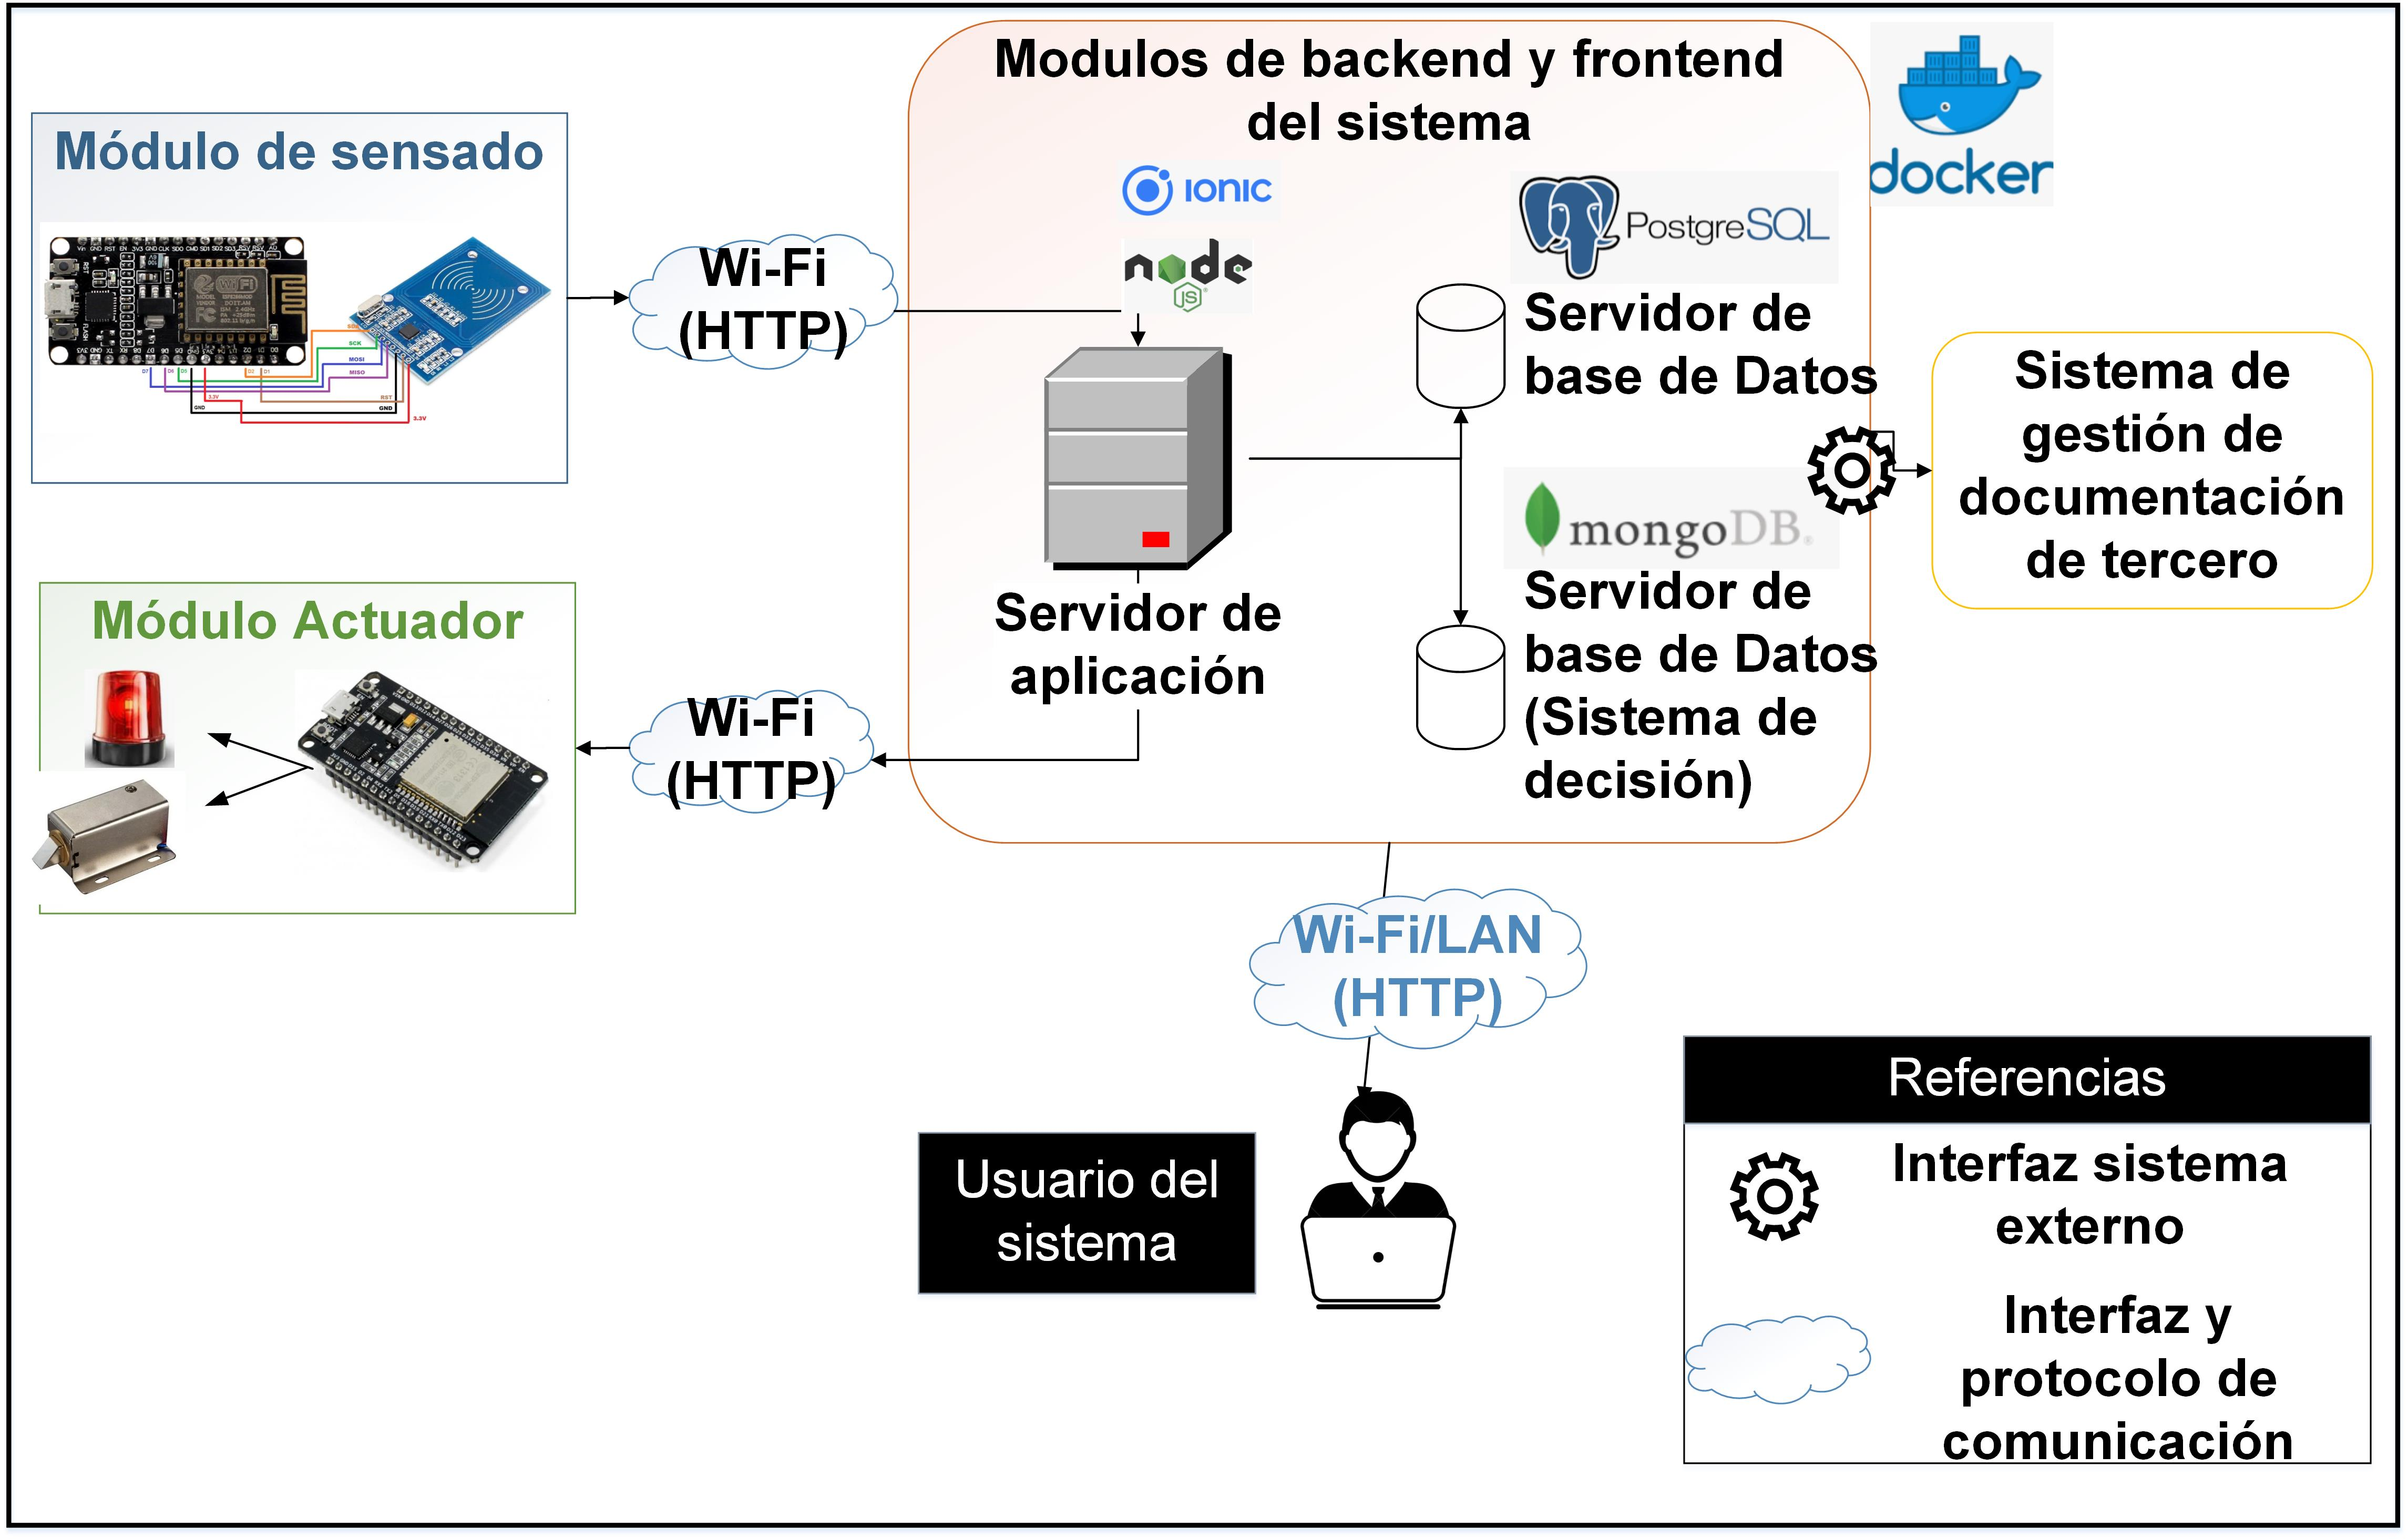
\includegraphics[width=1\textwidth]{./Figures/tp-final-infra.jpg}
	\caption{Diagrama en bloques del sistema implementado.}
	\label{fig:tp-final-infra}
\end{figure}

\pagebreak
\subsection{Módulos del sistema}

El trabajo desarrollado se divide en los siguientes módulos:

\begin{itemize}
\item Módulo de sensado: es el encargado de leer la tarjeta RFID y enviar la información al módulo de backend para analizar si la persona cumple con los requisitos para acceder o no.
\item Módulo actuador: es el encargado de comandar la cerradura electrónica que permite o evita el ingreso del tercero a la locación industrial. El mismo recibe las órdenes de cómo operar desde el módulo de backend.
\item Módulos de backend y frontend: si bien estos módulos están implementados de manera conjunta en un único servidor de aplicación, cumplen funciones diferentes:

	\begin{itemize}
	\item Módulo de frontend: es el encargado de brindar una interfaz gráfica a los usuarios, para que estos puedan interactuar con la aplicación, recibiendo sus solicitudes y proporcionándoles la información en un formato simple.
	\item Módulo de backend: es quien gestiona todas las solicitudes provenientes del módulo de sensado y del módulo de frontend. Es el encargado de analizar las solicitudes y responder a las mismas. Cuando recibe peticiones del frontend responde al mismo. Cuando recibe peticiones del módulo de sensado, actúa enviándole órdenes o comandos al módulo actuador. También es el encargado de comunicarse con el sistema de gestión de documentación de terceros. Para cumplir con sus funciones utiliza información almacenada en los servidores de base de datos.
	\end{itemize}
\item Sistema de gestión de documentación de terceros: este sistema es externo y no fue parte del desarrollo. El módulo de backend utiliza el mismo para obtener información de los terceros y en base a ésta tomar las decisiones de habilitar o inhabilitar el acceso y generar alertas y tareas de control.
\end{itemize}

\subsection{Protocolos de comunicación entre módulos}
Para la comunicación entre los módulos se utilizaron invocaciones HTTP GET y POST. 
Tomando como referencia el modelo TCP/IP \citep{WEBSITE:modeloTCPIP}, en la tabla \ref{tab:protocolosComunicacionCap3} se muestra el detalle de protocolos empleados en cada capa:


\begin{table}[h]
	\centering
	\caption[Protocolos comunicación empleados por el sistema]{Protocolos de comunicación empleados por el sistema.}
	\begin{tabular}{p{3.5cm} p{8.5cm} } 	

		\toprule
		\textbf{Capa del modelo} & 
		\textbf{Protocolo}
		\\
		\midrule

Aplicación & HTTP (utilizando los verbos GET y POST)\\ 
Transporte & TCP\\
Internet & IP (IPv4)\\
Acceso al medio &
\begin{itemize}
\item Wi-Fi (802.11n) para la comunicación entre módulos
\item Wi-Fi o IEEE 802.3 (Ethernet) para la comunicación entre el usuario y el módulo de frontend
\end{itemize} \\



		\bottomrule
		\hline
	\end{tabular}
	\label{tab:protocolosComunicacionCap3}
\end{table}

Para la elección de los protocolos, se tomó en cuenta las tecnologías disponibles en la empresa. Además, al utilizar protocolos abiertos, estándares y extendidos mundialmente, se logró un sistema portable y adaptable.

\pagebreak
\subsection{Tecnologías de bases de datos}

El sistema en general y el módulo de backend en particular, se soporta en dos bases de datos:

\begin{itemize}
\item Una base de datos relacional, implementada en PostgreSQL, que es la que contiene todos los objetos necesarios para la aplicación: usuarios, sensores, actuadores, terceros, eventos del sistema, tareas y sub-tareas de control. 
\item Una base de datos no relacional, implementada en MongoDB, que es utilizada por el backend para almacenar la relación entre los eventos de entrada y el conjunto de acciones que se deben tomar en función de dichos eventos. La decisión de utilizar una base no relacional se debe a que cada tipo de evento de entrada genera diferentes tipos de acciones de salida. Por ejemplo, en el caso de un evento de ingreso de un tercero con documentación en regla solo se debe realizar una acción de apertura de cerradura para el módulo actuador. Pero para un evento de ingreso con documentación vencida se deben generar acciones para cerrar la cerradura en el módulo actuador, generar tareas de control para diferentes sectores de planta y enviar un mail a las personas definidas por la gerencia de la empresa. 

\end{itemize}

\subsection{Contenedores docker y escalamiento}

A fin de generar una solución escalable y modular, se utilizaron contenedores docker para implementar el módulo de backend, el módulo de frontend y para levantar las instancias de base de datos, tanto PostgreSQL como MongoDB. Esta decisión permitió:

\begin{itemize}
\item Simplificar el \textit{deploy} de la aplicación: facilitando la configuración del servidor o servidores donde se ejecuta el sistema.
\item Lograr la escalabilidad futura de la solución: al permitir utilizar un orquestador de contenedores como Kubernetes que permite crear o eliminar instancias de cada contenedor dinámicamente en función de diferentes variables, como el consumo de recursos o la cantidad de solicitudes por segundo. Una ventaja adicional es que, si migramos la solución a la nube, al utilizar este esquema de contenedores dinámicos podemos reducir el costo del servicio, dado que estaremos pagando solo por los contenedores que necesitamos en cada instante de tiempo, sin necesidad de tener un número fijo de recursos en todo momento.
\end{itemize}

\section{Detalle de módulos de hardware}

En esta sección se describe detalladamente la implementación de los dos módulos de hardware desarrollados en el trabajo. El módulo sensor, encargado de la lectura de las tarjetas RFID del personal de tercero, y el módulo actuador, encargado de gestionar la cerradura electrónica para permitir o evitar el ingreso de dicho personal.

\subsection{Módulo sensor}

Es el encargado de leer las tarjetas RFID y enviar el valor que tiene la misma al módulo de backend.

Cada tarjeta RFID tiene un valor numérico guardado de 4 caracteres de longitud. Las tarjetas permiten definir valores de hasta 16 caracteres, pero dado que la empresa utiliza códigos de 4 caracteres se colocó ese límite para tener uniformidad.

El módulo está compuesto por los siguientes componentes:

\begin{itemize}
\item Un lector de tarjetas RFID RC522. La elección del mismo se debió a su bajo costo, alta disponibilidad en el mercado y su capacidad para leer las tarjetas que tiene la empresa, que operan en la frecuencia de 13,56 MHz.
\item Un \textit{SoC} (System on a chip) ESP32-WRROM-32. La elección del mismo se debió a su bajo costo, alta disponibilidad en el mercado, facilidad de programación y soporte de redes Wi-Fi (normas 802.11 b/g/n). Esto último simplifica la comunicación del módulo con el backend y evita tener que conectarse a la red LAN de la empresa, lo que hubiera requerido hacer una extensión del cableado de la misma.
\item Un conjunto de leds. Permite al usuario conocer el estado del sistema y el estado de sus interacciones con el módulo. Para ello se dispuso un grupo de 3 leds generales de control y otro de 3 leds de respuesta ante las comunicaciones con el backend.

\end{itemize}

En la figura \ref{fig:moduloSensor} se muestra el módulo sensor junto a sus componentes.

\begin{figure}[ht]
	\centering
	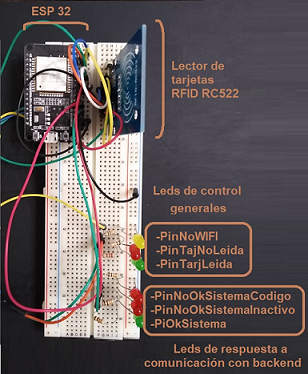
\includegraphics[width=0.8\textwidth]{./Figures/moduloSensor.png}
	\caption{Módulo sensor junto a sus componentes.}
	\label{fig:moduloSensor}
\end{figure}

\clearpage
\subsubsection{Configuraciones y variables del módulo}

Para implementar este módulo, se desarrolló un programa en el entorno Arduino IDE. El mismo lee las tarjetas RFID y se comunica con el backend, enviando los datos requeridos para procesar el intento de ingreso. Dicha comunicación se realiza a través de la red Wi-Fi de la empresa.


El módulo cuenta con un conjunto de variables a configurar para su correcta operación:

\begin{itemize}
\item WIFI\_SSID: especifica el SSID de la red Wi-Fi de la empresa.
\item WIFI\_PASSWORD: especifica el password de la red Wi-Fi de la empresa.
\item ID\_SENSOR: especifica el ID que tiene el sensor en la base de datos del sistema. Los datos de cada sensor se almacenan en dicha base de datos, la cual incluye su estado, descripción, ubicación y token asociado.
\item tokenlocal: especifica el token de 20 caracteres que tiene asociado el sensor en la base de datos. Con este valor se asegura la autenticación del módulo.
\item servicioAPISensor: contiene la URL del endpoint que expone el backend para recibir los datos de este módulo.
\end{itemize}

\subsubsection{Comunicación con el backend}

El módulo tiene configurada la dirección URL del endpoint que el backend expone para permitir la comunicación entre éstos.

Para enviar los datos solicitados, se realiza un HTTP POST con un objeto JSON que tiene 3 claves:

\begin{itemize}
\item id: contiene el valor ``ID\_SENSOR'' del módulo.
\item token: contiene el valor de ``tokenlocal'' del módulo.
\item valor: contiene el valor leído de la tarjeta RFID, que representa al id del tercero en el sistema.
\end{itemize}

Una vez enviado el HTTP POST, el módulo recibe como respuesta un valor que indica si los datos mandados son correctos o si hubo algún error. Con esta respuesta se determina qué leds deben activarse para dar \textit{feedback} al usuario del estado del proceso.

\subsubsection{Leds del sistema}

El módulo cuenta con un conjunto de leds, que permiten al usuario conocer el resultado de sus interacciones con éste.

Al inicializar el módulo se realiza un chequeo de estos leds, prendiéndolos y apagándolos, uno a uno, durante medio segundo.

En la tabla \ref{tab:combinacionLedsSensor} se muestra el detalle de los leds o combinaciones posibles de leds, junto a la información que brindan al usuario cuando se encienden.

\begin{table}[h]
	\centering
	\caption[Leds del módulo sensor]{Combinación de leds e información para el usuario cuando se prenden.}
	\begin{tabular}{p{4cm} p{8.5cm} } 	

		\toprule
		\textbf{Led/combinación de leds} & 
		\textbf{Información para el usuario}
		\\
		\midrule

PinNoWIFI & Al leer la tarjeta del tercero, si no se cuenta con comunicación Wi-Fi con el backend, el led se prende durante 3 segundos.\\ 
PinTarjNoLeida & Falló la lectura de la tarjeta o la misma no tiene valor asignado. Se debe configurar la tarjeta con el valor correspondiente al personal de tercero.\\
PinTarjLeida & Al acercar la tarjeta al lector, el sistema lee correctamente la misma, junto al valor que tiene almacenado.\\
PinOkSistema & Una vez leída la tarjeta del personal de tercero, el sistema se comunica correctamente con el backend. Se informa al usuario al prender el led durante 2 segundos. \\
PinNoOkSistemaCodigo & Una vez leída la tarjeta del personal de tercero, el sistema se comunica correctamente con el backend, pero el valor de ``ID\_SENSOR'' enviado no se corresponde con ningún módulo sensor configurado en el sistema, o el mismo está inactivo. Se informa al usuario al prender el led durante 2 segundos. \\
PinNoOkSistemaCodigo
+
PinNoOkSistemaInactivo & Una vez leída la tarjeta del personal de tercero, el sistema se comunica correctamente con el backend, pero éste devuelve un error con un código no especificado. Se informa al usuario al prender el ``led PinNoOkSistemaCodigo'' durante 1 segundo seguido del led ``PinNoOkSistemaInactivo'' durante otro segundo.
\\
		\bottomrule
		\hline
	\end{tabular}
	\label{tab:combinacionLedsSensor}
\end{table}


\subsection{Módulo actuador}

Es el encargado de comandar la cerradura. El mismo cuenta con un conjunto de leds que brindan información al personal de tercero del estado del módulo y del estado de su ingreso.

Las órdenes de cómo operar las recibe desde el módulo de backend, para lo cual el actuador expone un \textit{endpoint} HTTP, que recibe un JSON con dichas órdenes.

\pagebreak
El módulo está compuesto por los siguientes componentes:

\begin{itemize}
\item Un \textit{SoC} ESP32-WRROM-32. La elección del mismo se debió a su bajo costo, alta disponibilidad en el mercado, facilidad de programación y soporte de redes Wi-Fi (normas 802.11 b/g/n). Esto último simplifica la comunicación del módulo con el backend y evita tener que conectarse a la red LAN de la empresa, lo que hubiera requerido hacer una extensión del cableado de la misma.
\item Un regulador de tensión. Brinda los niveles de tensión requeridos para energizar el ESP32 y para la activación del Mosfet IRF520. 
\item Cerradura electrónica. La misma se acciona y alimenta desde el Mosfet IRF520.
\item Conversor de niveles lógicos. Se utiliza para convertir la tensión de salida del ESP32 (3.3 V) a la tensión requerida para accionar el Mosfet IFR520 (5V).
\item Mosfet IRF520. Permite accionar la cerradura electrónica, brindando el nivel de tensión requerida por la misma (12 V).
\item Un conjunto de leds. Permiten conocer si el actuador está encendido y el estado del ingreso del tercero (habilitado/inhabilitado/error).
\item Fuente de alimentación de 12 V. Es utilizada para alimentar el  Mosfet IRF520 y al regulador de tensión.
\end{itemize}

En la figura \ref{fig:moduloActuador} se muestra el módulo actuador con sus componentes.

\begin{figure}[ht]
	\centering
	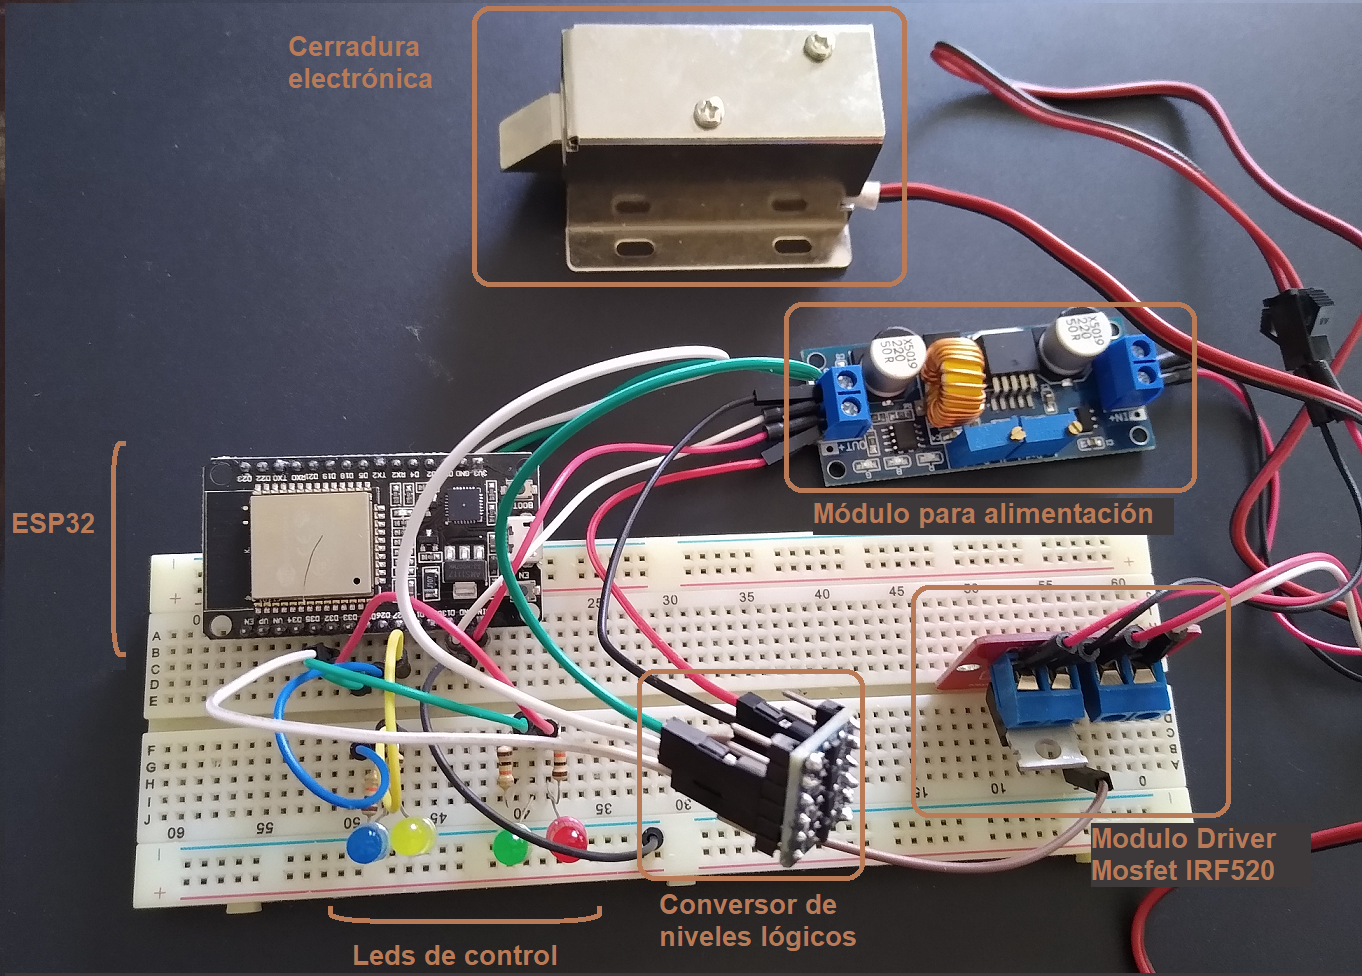
\includegraphics[width=1\textwidth]{./Figures/moduloActuador.png}
	\caption{Módulo actuador junto a sus componentes.}
	\label{fig:moduloActuador}
\end{figure}

\subsubsection{Configuraciones y variables del módulo}

Para implementar el actuador, se desarrolló un programa en el entorno Arduino IDE. Este programa expone un \textit{endpoint} HTTP POST, que recibe un JSON con las acciones a realizar. En función de la acción y valor indicados, se acciona la cerradura electrónica y se prenden los leds de control.

En la base de datos del sistema se guarda la información de los actuadores existentes, su ubicación, descripción, estado, dirección IP y token de autenticación.

El actuador cuenta con un conjunto de variables a configurar para su correcta operación:

\begin{itemize}
\item WIFI\_SSID: especifica el SSID de la red Wi-Fi de la empresa.
\item WIFI\_PASSWORD: especifica el password de la red Wi-Fi de la empresa.
\item tokenlocal: especifica el token de 20 caracteres que tiene asociado el actuador en la base de datos. Con este valor se asegura la autenticación del módulo.
\item local\_IP: especifica la dirección IP del mismo. Se utiliza una IP fija, para asegurar que el \textit{endpoint} expuesto siempre pueda ser accedido. Si se utilizara una IP dinámica la dirección podría cambiar y quedaría inaccesible dicho \textit{endpoint}.
\item Subnet: dirección de sub-red de la red Wi-Fi.
\end{itemize}

\subsubsection{Comunicación desde el backend}

El módulo recibe un HTTP POST desde el backend con un objeto JSON que tiene 3 claves:

\begin{itemize}
\item token: contiene el token de autenticación.
\item acción: contiene la acción a realizar. Es un clasificador de acciones posibles.
\item valor: contiene el valor particular para la acción.
\end{itemize}

Al recibir el objeto se controla si el token coincide con el valor de token que se tiene almacenado localmente, y luego se controla si la acción y valor son válidos. En función de la acción y valor, se abre o cierra la cerradura, y prende el led de ingreso ok, de ingreso no ok o de error. Por último, se responde al backend con un código de error o un ok.

\subsubsection{Detalle de respuestas ante solicitudes del backend}

El backend realiza solicitudes al actuador como se explica en la sub-sección anterior. En la tabla \ref{tab:respuestasActuadorBackend} se muestra el detalle las diferentes combinaciones de valores que puede recibir el módulo en las solicitudes y se indica la respuesta brindada al usuario y al backend.


\begin{table}[h]
	\centering
	\caption[Respuestas posibles del módulo al usuario y al backend ante las solicitudes recibidas]{Respuestas posibles del módulo al usuario y al backend ante las solicitudes recibidas.}
	\begin{tabular}{p{4cm} p{4.5cm} p{4.5cm} } 	

		\toprule
		\textbf{Valores recibidos} & 
		\textbf{Respuesta al usuario} &
		\textbf{Respuesta al backend} 
		\\
		\midrule

Acción=``APERTURA''

Valor=``ABRIR''

Token con valor correcto.& Se prende el led verde de manera intermitente durante 4 segundos. Durante ese tiempo la cerradura electrónica se cierra. & Se envía respuesta HTTP con código 200 y mensaje OK. \\
Acción=``APERTURA''

Valor=``CERRAR''

Token con valor correcto. & Se prende el led rojo durante 2 segundos. & Se envía respuesta HTTP con código 200 y mensaje ``Sin token de autenticación.''. \\
Sin token. & Se prende el led amarillo  durante medio segundo y se apaga. & Se envía respuesta HTTP con código 401 y mensaje ``Sin token de autenticación.''. \\
Token con valor incorrecto. & Se prende el led amarillo  durante medio segundo y se apaga. & Se envía respuesta HTTP con código 403 y mensaje ``Token de autenticación incorrecto.''. \\
Acción no especificada o con valor incorrecto. & Se prende el led amarillo de manera intermitente durante 2 segundos. & Se envía respuesta HTTP con código 400 y mensaje ``La acción especificada no es válida.''. \\
Valor no especificado o valor incorrecto. & Se prende el led amarillo de manera intermitente durante 3 segundos. & Se envía respuesta HTTP con código 400 y mensaje ``El valor especificado no es válido''. \\
		\bottomrule
		\hline
	\end{tabular}
	\label{tab:respuestasActuadorBackend}
\end{table}

\pagebreak
\section{Detalle de módulos de software}

En esta sección se describe detalladamente la implementación de los dos módulos de software desarrollados en el trabajo: el de backend, encargado tanto de recibir las solicitudes del módulo sensor y de frontend como de enviar comandos al actuador, y el módulo de frontend, encargado de gestionar las solicitudes del usuario mediante una interfaz gráfica.

\subsection{Módulo de backend}

El mismo está implementado como una aplicación web con Node.JS, utiliza las librerías Express y Socket.io y expone:

\begin{itemize}
\item Una API Rest para el frontend, la cual responde a sus solicitudes e incluye un WebSocket para mostrar alertas online a la Portería.
\item Una API de autenticación, utilizada para la gestión e inicio de sesión de los usuarios.
\item Un \textit{endpoint} para recibir las solicitudes de ingreso del módulo sensor.
\end{itemize}

Para su desarrollo se utilizó el IDE Visual Studio Code. Dentro del mismo se organizaron las carpetas con el código y las configuraciones para el testing automático.

En la figura \ref{fig:backendCarpetas}  se muestra la estructura en carpetas definidas para el backend.

\begin{figure}[ht]
	\centering
	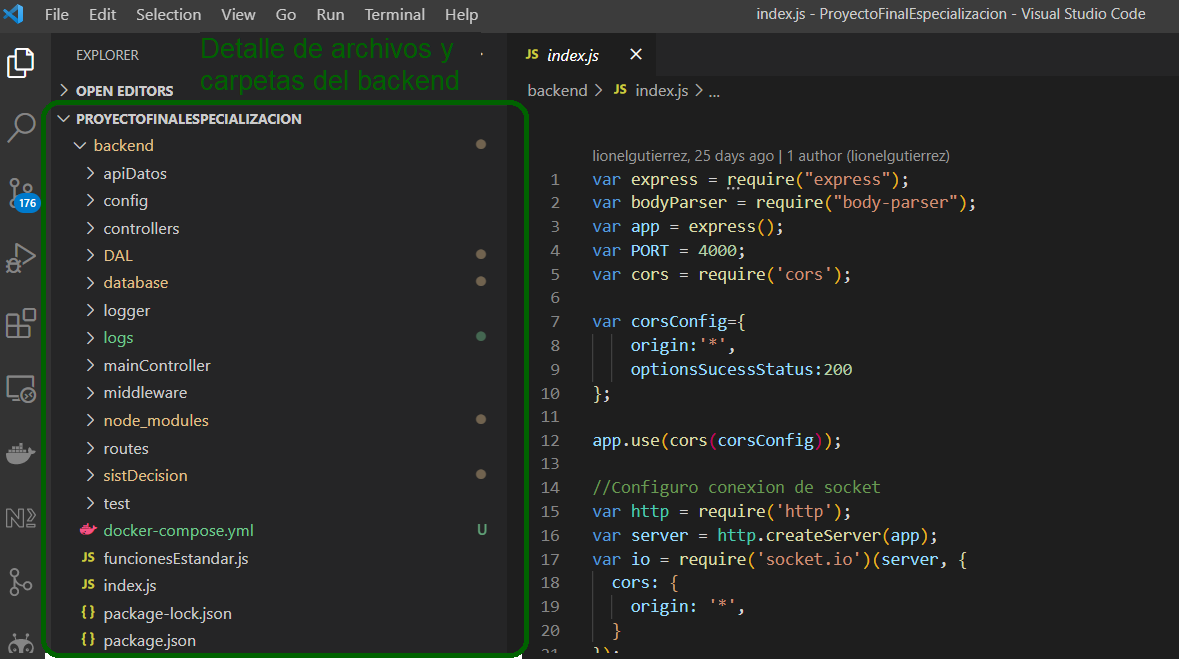
\includegraphics[width=1\textwidth]{./Figures/backendCarpetas.png}
	\caption{Estructura de directorio del backend desarrollado en Visual Studio Code.}
	\label{fig:backendCarpetas}
\end{figure}

En la tabla \ref{tab:carpetasBackend}  se expone detalladamente el contenido y función de cada una de las carpetas y archivos del módulo.

\begin{table}[h]
	\centering
	\caption[Detalle de archivos y carpetas del módulo de backend]{Detalle de archivos y carpetas del módulo de backend.}
	\begin{tabular}{p{2cm} p{11cm}} 	
		\toprule
		\textbf{Archivo/
		Directorio} & 
		\textbf{Descripción} 
		\\
		\midrule
apiDatos & Contiene cada uno de los \textit{endpoints} expuestos al frontend. Se implementó utilizando Express, junto a métodos GET y POST, para servir las consultas de información y las altas y actualizaciones en la base de datos. \\
config & Contiene tanto la configuración del \textit{secret} necesaria para el sub-módulo de autenticación, como la configuración de constantes utilizadas en la comunicación con el sistema de documentación de terceros. \\
controllers & Cuenta con tres controladores:
\begin{itemize}
\item generacionAlertas: es el encargado de comunicarse con el módulo actuador y enviarle los comandos para habilitar o prohibir la solicitud de ingreso del tercero a la planta.
\item generacionMensajes: es el encargado de gestionar el envío de emails a los usuarios requeridos.
\item generacionTareas: es el encargado de generar las tareas y sub-tareas, guardando la información en la base de datos.
\end{itemize} \\
DAL & La DAL (Data Access Layer), es la encargada de abstraer la comunicación con la base de datos, al brindar un conjunto de métodos para acceder y realizar las altas, bajas y modificaciones, sin necesidad de que los componentes que la usan conozcan la implementación subyacente. \\
database & Contiene las configuraciones necesarias para conectarse a la base de datos PostgreSQL. Se utiliza un \textit{pool} de conexiones a fin de mejorar el rendimiento y la escalabilidad del sistema. \\
logger & Es el encargado de gestionar el \textit{logging} de eventos.\\
logs & Almacena los \textit{logs} del sistema. Se guarda un archivo de \textit{log} por día para evitar archivos muy extensos y simplificar la búsqueda de información en los mismos. \\
main

Controller & Es el encargado de gestionar las solicitudes de ingreso del módulo sensor. Se comunica con el sistema de documentación de terceros, determina los tipos de acción a realizar y dispara cada una de ellas, invocando a los controladores de la carpeta controllers.  \\
middleware & Contiene los métodos necesarios para la gestión de la autenticación. \\
routes & Contiene cada uno de los \textit{endpoints} expuestos tanto para la API de autenticación (sub-carpeta ``routerAuth'') como para la recepción de datos desde el módulo sensor (sub-carpeta ``routerSensores''). \\
sistDecision & Contiene el sub-módulo que se encarga de determinar las acciones a realizar cuando hay una solicitud de ingreso de un tercero, para lo cual utiliza la base de datos implementada en MongoDB. \\
test & Contiene los archivos necesarios para la ejecución de las pruebas automáticos implementados para la solución. En el capítulo \ref{Chapter4} se explican con mayor detalle las pruebas implementadas y los archivos utilizados. \\
index.js & Contiene la configuración para levantar la aplicación y cada una de las rutas utilizadas por la aplicación. También incluye la configuración de CORS y del WebSocket. \\
		\bottomrule
		\hline
	\end{tabular}
	\label{tab:carpetasBackend}
\end{table}

\clearpage
\subsubsection{API de autenticación}

La API de autenticación se utiliza para segurizar las invocaciones realizadas al backend. Para hacerlo emplea tokens JWT. Además, permite el alta de nuevos usuarios, gestionar el inicio de sesión de los mismos y el cambio y reseteo de passwords.

Para el desarrollo de esta API se utilizan 2 librerías disponibles en node.JS: bcryptjs y jsonwebtoken. La primera permite implementar una función de \textit{hash}, que posibilita guardar encriptado el password de los usuarios. La segunda permite generar el token JWT que es entregado al usuario para que pueda acceder a los diferentes \textit{endpoints}, asegurando su autenticidad. Dicho token tiene una duración de 24 horas.

\subsubsection{Funcionamiento del módulo ante una solicitud del módulo sensor}{\label{sec:subSeccionSolitiudModuloSensor}}   

Cuando el módulo sensor hace una solicitud al backend invoca al \textit{endpoint} de recepción de sensores. El backend, por su parte, recibe la solicitud y realiza los pasos descriptos a continuación: 

\begin{enumerate}
\item Envía el pedido al router ``routerSensores''. 
\item ``routerSensores'' controla el token y valores recibidos. Si el token no es válido o el id de sensor enviado no es correcto o está inactivo, se envía un mensaje de error al origen y se termina la solicitud.
\item Si los datos son correctos, se envían al ``mainController''.
\item El ``mainController'' realiza estas acciones:
	\begin{enumerate}
	\item Se comunica con el sistema de documentación de terceros para determinar si la persona está en condiciones de ingresar. 
	\item Registra el evento de ingreso en la base de datos (no directamente, sino a través de la ``DAL'').
	\item Con los datos obtenidos se comunica con el sub-módulo de decisión (``sistDecision''), el cual le indica las acciones a realizar. 
	\item Para cada una de las acciones indicadas, en función del tipo que sea (de salida, mensaje, tarea), se comunica con los controladores ``generacionAlertas'', ``generacionMensajes'' o ``generacionTareas'', para que éstos las procesen y registren.
	\end{enumerate}
\end{enumerate}

En la figura \ref{fig:DiagramaInteaccion1} se muestra la interrelación entre los componentes del módulo y el flujo de datos ante una solicitud desde el módulo sensor.

\begin{figure}[ht]
	\centering
	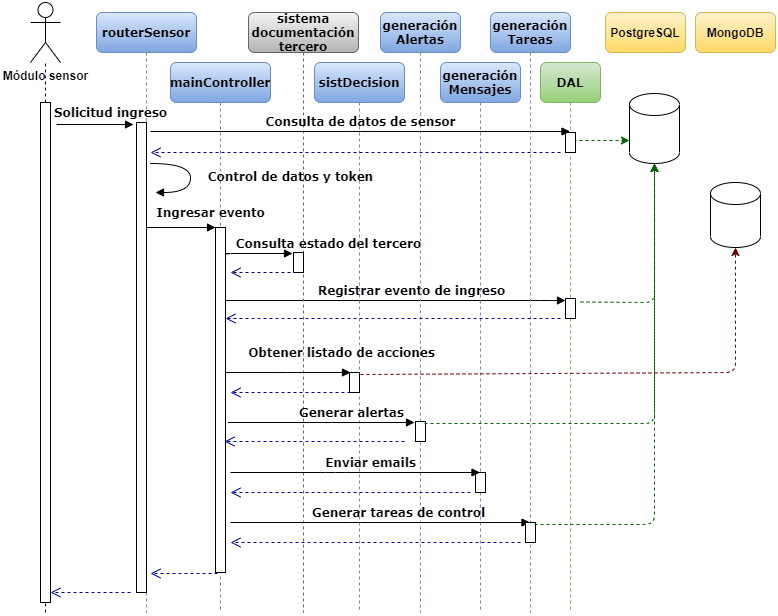
\includegraphics[width=1\textwidth]{./Figures/DiagramaInteaccion1.png}
	\caption{Interacción entre los componentes del módulo ante una solicitud del módulo sensor.}
	\label{fig:DiagramaInteaccion1}
\end{figure}

\pagebreak
\subsubsection{Funcionamiento del módulo ante una solicitud del módulo de frontend}

Cuando el módulo de frontend hace una solicitud al backend invoca algunos de los \textit{endpoints} definidos en ``apiDatos''. El backend, por su parte, recibe la solicitud y realiza los pasos descriptos a continuación: 
\begin{enumerate}
\item Envía el pedido a ``apiDatos''. 
\item ``apiDatos'' determina el endpoint solicitado, pasa el control al mismo y éste realiza las siguientes acciones:
	\begin{enumerate}
	\item Controla que la solicitud tenga el token de autenticación y lo valida utilizando las funciones del \textit{middleware} de autenticación.
	\item Si el token no es correcto se rechaza el pedido con un código 403.
	\item Si el token es correcto, opcionalmente y según la necesidad de cada \textit{endpoint}, controla el rol de usuario asociado al token utilizando nuevamente el \textit{middleware} de autenticación.
	\item Si el rol/roles solicitados no son correctos rechaza el pedido con un código 403.
	\item Si los roles son correctos procede con la solicitud. En general cada solicitud controla los datos de entrada y luego se comunica con la base de datos a través de la ``DAL'', ya sea para consultar, agregar o modificar información.
	\end{enumerate}

\end{enumerate}

En la figura \ref{fig:DiagramaInteraccion2} se muestra la interrelación entre los componentes del módulo y el flujo de datos ante una solicitud desde el frontend.

\begin{figure}[ht]
	\centering
	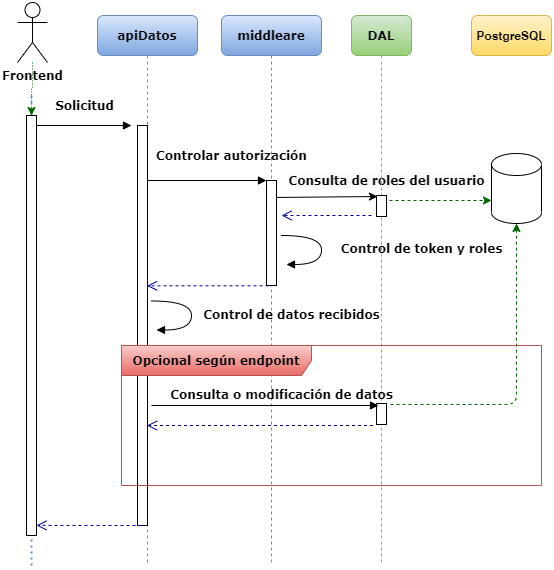
\includegraphics[width=1\textwidth]{./Figures/DiagramaInteraccion2.png}
	\caption{Interacción entre los componentes del módulo ante una solicitud del frontend.}
	\label{fig:DiagramaInteraccion2}
\end{figure}

\subsection{Módulo de frontend}

Este módulo brinda una interfaz gráfica al usuario a través de la cual interactúa con el sistema, ya sea para consultar datos o para registrar acciones. Con el objetivo de cumplir con tales funciones se comunica con el backend a través de una API Rest. Para su desarrollo se empleó Angular y el framework Ionic. Su utilización permitió construir el sistema como una aplicación web responsive con la idea de implementarla a futuro como una \textit{app mobile}. Para la escritura del código fuente apelamos al IDE Visual Studio Code. Dentro del mismo se organizaron las carpetas con el código y cada uno de los diferentes elementos.

\pagebreak
En la figura \ref{fig:frontendCarpetas} se muestra la estructura en carpetas definidas para el frontend.

\begin{figure}[ht]
	\centering
	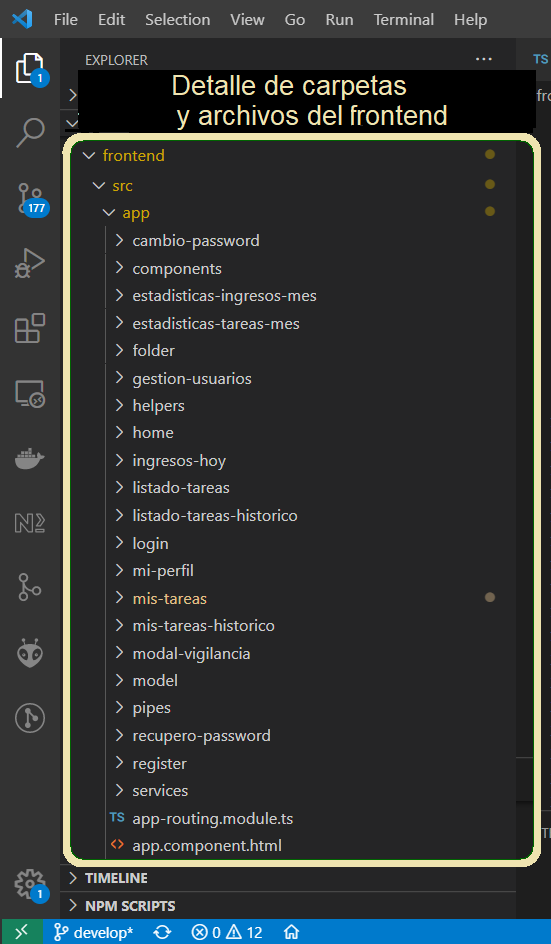
\includegraphics[width=.6\textwidth]{./Figures/frontendCarpetas.png}
	\caption{Estructura de directorio del frontend desarrollado en Visual Studio Code.}
	\label{fig:frontendCarpetas}
\end{figure}


En la tabla \ref{tab:carpetasFrontend}  se expone detalladamente el contenido y función de cada una de las carpetas y archivos del módulo.

\begin{table}[h]
	\centering
	\caption[Detalle de archivos y carpetas del módulo de frontend]{Detalle de archivos y carpetas del módulo de frontend.}
	\begin{tabular}{p{2.3cm} p{10.7cm}} 	
		\toprule
		\textbf{Archivo/
		Directorio} & 
		\textbf{Descripción} 
		\\
		\midrule
cambio-password & Contiene la página que gestiona el cambio de password de los usuarios. \\
\hline
components & Contiene tres sub-carpetas con los componentes desarrollados para la solución. Los componentes implementados son:
\begin{itemize}
\item estadística-evento-fecha: muestra la cantidad de ingresos habilitados y rechazados en el día.
\item listar-tareas: muestra una grilla con el listado de tareas y sub-tareas en un rango de fechas y con un estado particular. 
\item tareas-usuario: muestra un listado con cada una de las sub-tareas que tiene un usuario.
\end{itemize} \\
\hline
estadísticas-ingreso-mes & Contiene la página que muestra las estadísticas de cantidad de ingresos por mes.\\
\hline
estadisticas-tareas-mes & Contiene la página que muestra las estadísticas de cantidad de tareas cerradas por año.\\
\hline
gestión-usuarios & Contiene la página que muestra el listado de usuarios del sistema y permite cambiar el estado de los mismos (activo/inactivo) y agregarles o quitarles roles. \\
\hline
helpers & Contiene la clase ``authInterceptor'' que permite enviar cada solicitud al backend con el token de autenticación. Para esto intercepta el pedido HTTP y le agrega al encabezado dicho token. \\
\hline
home & Contiene la página principal de la aplicación que muestra, según el rol del usuario, las estadísticas de ingreso al sistema o las tareas en curso del mismo.\\
\hline
ingresos-hoy & Contiene la página que muestra el listado de ingresos del día con la fecha de cada ingreso y si el usuario fue habilitado o no. \\
\hline
listado-tareas & Contiene la página que muestra el listado de tareas en curso. Utiliza el componente ``listar-tareas''. \\
\hline
listado-tareas
-historico & Contiene la página que muestra el listado de tareas completas. Utiliza el componente ``listar-tareas''. \\
\hline
login & Contiene la página de inicio de sesión para los usuarios. \\
\hline
mi-perfil & Contiene la página que muestra el perfil de usuario y sus datos. \\
\hline
mis-tareas & Contiene la página que muestra las tareas en curso asignadas al usuario. \\
\hline
mis-tareas
-historico & Contiene la página que muestra las tareas cerradas del usuario. \\
\hline
model & Contiene las clases que representan a los objetos de negocio del sistema: roles, usuarios, tareas, sub-tareas, sectores. \\
\hline
pipes & Contiene la implementación de un \textit{pipe}, que define diferentes colores en función del valor de entrada recibido. Sirve para alertar al usuario de la antigüedad de sus tareas. \\
\hline
recupero-password & Contiene la página que permite al usuario recuperar su password. \\
\hline
register & Contiene la página que permite dar de alta nuevos usuarios al sistema. \\
\hline
services & Contiene los servicios que utilizan las diferentes páginas y componentes para gestionar sus datos y consultas al backend. \\
		\bottomrule
		\hline
	\end{tabular}
	\label{tab:carpetasFrontend}
\end{table}

\clearpage
\subsubsection{Detalle de servicios (``services'') implementados}
En esta sub-sección se detallan los servicios implementados en Angular. Mientras que los componentes y las páginas están enfocados en brindar una interfaz gráfica simple y fácil de utilizar para los usuarios, los servicios se orientan a las tareas de lógica de negocio, lo que incluye comunicarse con el backend y gestionar la autenticación y los datos del usuario.

Los servicios implementados son los siguientes:

\begin{itemize}
\item authService: se comunica con la API de autenticación del backend para gestionar los inicios de sesión, el alta de nuevos usuarios y las funcionalidades de recuperación y cambio de password.
\item camibioMenuService: se encarga del armado del menú de aplicaciones del usuario, en función de su rol. 
\item datosAuxiliaresService: se encarga de comunicarse con el backend para consultar los datos auxiliares del sistema que son de acceso público como, por ejemplo, el listado de sectores de planta para la pantalla de alta de nuevos usuarios.
\item ingresosService: se comunica con el backend para obtener la información de ingresos a planta por rango de fechas.
\item socketService: gestiona el socket utilizado para que la vigilancia y la gerencia puedan visualizar en tiempo real los ingresos a la planta.
\item tareaService: se comunica con el backend para obtener información de las tareas en curso, de las tareas cerradas y para realizar modificaciones en las mismas.
\item tokenStorageService: es el encargado de la gestión del token de autenticación que devuelve el backend al iniciar sesión. Dentro de la gestión se incluye su almacenamiento y recuperación.
\item usuariosService: se comunica con el backend para realizar cambios en el estado de los usuarios y sus roles. Solo es utilizado por el rol administrador. 
\item loginGuardService: permite al módulo de ruteo de la aplicación controlar que el usuario cuente con el rol necesario para acceder a una determinada página. Este servicio se utiliza para habilitar los accesos a las páginas solo para el rol de usuario normal.
\item rolAdminGuardService: se utiliza para habilitar los accesos a las páginas solo para el rol de usuario administrador.
\item rolAGerenteGuardService: se utiliza para habilitar los accesos a las páginas solo para el rol de usuario gerente.
\item rolVigilanciaGuardService: se utiliza para habilitar los accesos a las páginas solo para el rol de usuario vigilancia.
\end{itemize}

\subsubsection{Funcionamiento del módulo ante un inicio de sesión}

En este apartado se explica el inicio de sesión de un usuario, en el que se puede ver la interacción con el backend y el guardado del token de autenticación para futuras consultas.
El proceso comienza cuando el usuario ingresa al sistema y visualiza la pantalla de inicio de sesión. Coloca su username y password y hace click en el botón “Loguearse”. Ante el click del usuario, el sistema realiza las siguientes interacciones:

\begin{enumerate}
\item El módulo ``loginModule'' invoca al servicio ``authService'' con los datos de username y password.
\item ``authService'' se comunica con el backend mediante un HTTP POST a la API de autenticación y recibe como respuesta el token asociado al usuario y los datos del mismo (username, password, email, sector y roles asociados). El servicio envía los datos recibidos al módulo ``loginModule''.
\item El módulo al recibir el token y los datos del usuario utiliza el servicio ``tokenStorageService'' para almacenar los valores. Luego, invoca al servicio ``cambioMenuService'' que genera el menú de usuario según sus roles. Por último, invoca al módulo ``homeModule'' que muestra la página de inicio al usuario. 
\end{enumerate}

En la figura \ref{fig:inisioSesionInteraccion} se muestra el diagrama de interacción para el inicio de sesión.

\begin{figure}[ht]
	\centering
	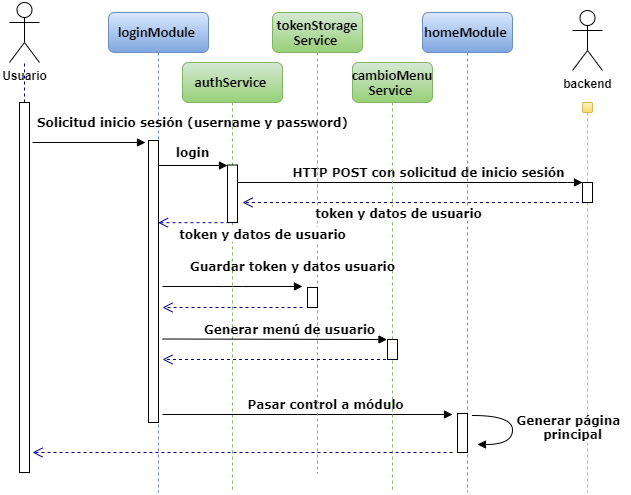
\includegraphics[width=1\textwidth]{./Figures/inisioSesionInteraccion.png}
	\caption{Diagrama de interacción para el inicio de sesión.}
	\label{fig:inisioSesionInteraccion}
\end{figure}

\pagebreak
\subsubsection{Funcionamiento del módulo ante una solicitud de usuario}

En esta sección se explica una interacción típica del usuario en la que se puede ver la relación entre los diferentes elementos del frontend y su comunicación con el backend.

Como pre-requisito, el usuario ya inició sesión en el sistema y desea consultar sus tareas en curso. Para ello hace click en la opción ``Mis Tareas en curso'' del menú de aplicaciones. Ante el click del usuario el sistema realiza las siguientes interacciones:

\begin{enumerate}
\item El módulo de ruteo ``app-routing.module'' determina quién es el encargado de procesar la solicitud del usuario. En nuestro caso es ``mis-tareas-module''. Luego, controla que éste pueda acceder a la página. Para ello consulta con el ``loginGuardService''.
\item Si se determina que se puede acceder a la página, se transfiere el control al módulo ``mis-tareas-module''. Éste invoca al servicio ``tokenStorageService'' para adquirir el token de usuario y su id. Con dicho id llama al servicio ``tareasService'' para obtener las tareas del usuario.
\item El servicio ``tareaService'' genera la solicitud HTTP GET y la envía al backend.
\item El ``authInterceptor'' intercepta la solicitud y le agrega un encabezado con el token de autenticación.
\item El backend procesa la solicitud y devuelve el listado de tareas en curso del usuario.
\item El servicio ``tareaService'' devuelve el listado al módulo ``mis-tareas-module''.
\item El módulo arma con el listado la pantalla necesaria para mostrar la información en un formato simple y la envía al usuario.
\end{enumerate}

En la figura \ref{fig:UsuarioPedidoInteraccion} se muestra el diagrama de interacción para una solicitud de usuario.

\begin{figure}[ht]
	\centering
	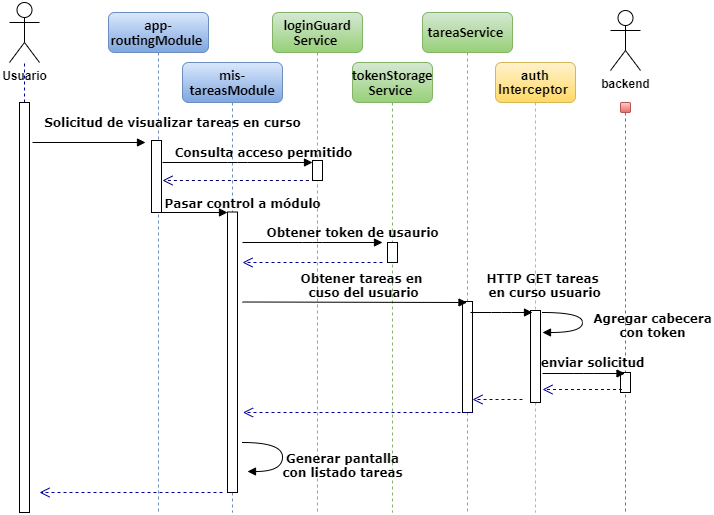
\includegraphics[width=1\textwidth]{./Figures/UsuarioPedidoInteraccion.png}
	\caption{Diagrama de interacción para una solicitud de usuario.}
	\label{fig:UsuarioPedidoInteraccion}
\end{figure}

\pagebreak
\subsubsection{Pantalla principal de vigilancia}

Para el rol de vigilancia se implementó un \textit{WebSocket} que posibilita una comunicación en tiempo real con el backend. Esto permite que ante los intentos de ingreso a planta del personal de tercero, el vigilante pueda tener al instante una alerta, ya sea de un acceso exitoso o de un acceso denegado. Para implementar dicho \textit{WebSocket} se utilizó la librería Socket.io, tanto en el backend como en el frontend. 

A continuación, se muestran los pasos que realiza el sistema y los componentes involucrados en la generación de una alerta:
\begin{enumerate}
\item Cuando el usuario de vigilancia inicia sesión en la aplicación, la misma lo redirige a su página principal (módulo ``homeModule''). En ese momento, el frontend utiliza el servicio ``socketService'' para iniciar el WebSocket con el backend y suscribirse a los eventos de tipo ``ingreso''.
\item Posteriormente, cuando un usuario de tercero intenta ingresar a planta, el backend recibe la solicitud de ingreso, la procesa y genera las tareas de control y alertas correspondientes, según lo explicado en la subsección \ref{sec:subSeccionSolitiudModuloSensor}. Dentro de dichas acciones, el sistema emite un evento del tipo ``ingreso'' que contiene el resultado del intento de acceso, los datos del tercero asociado y una descripción con el motivo de la habilitación o denegación.
\item El módulo ``homeModule'' recibe el evento del backend y genera la alerta al vigilante. La misma se presenta en un \textit{Pop up} que se muestra durante 6 segundos e incluye los detalles del acceso. Para ver el detalle de cada tipo de acceso referirse a la sección \ref{sec:PruebasAceptacion}
\end{enumerate}

En la figura \ref{fig:DiagramaInteraccionVigi} se muestra el diagrama de interacción para la pantalla de principal de vigilancia.

\begin{figure}[ht]
	\centering
	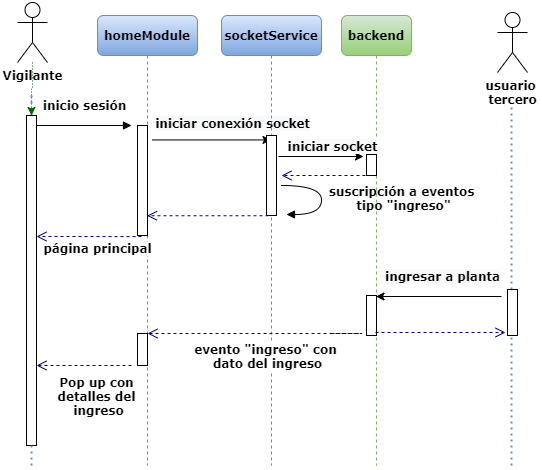
\includegraphics[width=1\textwidth]{./Figures/DiagramaInteraccionVigi.png}
	\caption{Diagrama de interacción para la pantalla de principal de vigilancia.}
	\label{fig:DiagramaInteraccionVigi}
\end{figure}

\section{Interfaz con sistema de documentación}

El sistema de documentación de terceros es un aplicativo que ya está desarrollado en la empresa. El acceso al mismo es a través de un \textit{endpoint} HTTP GET, al cual se le indica el id del usuario de tercero que se quiere consultar, y devuelve un objeto JSON con la información del nombre y apellido de la persona, si el acceso se debe permitir o no (variable con valor OK o NO) y el motivo por el cual se habilita o no al mismo. Para configurar el acceso a dicho sistema dentro de nuestro desarrollo, bastó con contar con la dirección del \textit{endpoint}. 

Dado que el desarrollo y las pruebas se realizaron en un entorno desconectado de la empresa, se implementó un \textit{mock} para simular el acceso al sistema. Dicho \textit{mock} se desarrolló como una aplicación web con Node.JS y la librería Express, lo que permitió exponer un \textit{endpoint} HTTP GET del mismo modo que lo hace el sistema original. Para el desarrollo se utilizó el IDE Visual Studio Code y se tomaron 4 casos típicos como respuesta:

\begin{enumerate}
\item Usuario activo con documentación en regla.
\item Usuario activo con documentación vencida.
\item Usuario dado de baja (fin de contratación).
\item Usuario no existente (id de usuario nunca dado de alta).
\end{enumerate}

Con estos 4 casos definidos se pudieron probar todas las alternativas y asegurar la respuesta correcta de nuestra aplicación.
